%%%%%%%%%%%%%%%%%%%%%%%%%%%%%%%%%%%%%%%%%%%%%%%%%%%%%%%%%%%%%%%%%%%%%%%%
%%%%%                                                              %%%%%
%%%%% Chapter 4: Identifying SMURF-seq fragment boundaries         %%%%%
%%%%%                                                              %%%%%
%%%%%%%%%%%%%%%%%%%%%%%%%%%%%%%%%%%%%%%%%%%%%%%%%%%%%%%%%%%%%%%%%%%%%%%%

\chapter{Identifying fragment boundaries on a SMURF-seq read}
\label{ch4}

%%%%%%%%%%%%%%%%%%%%%%%%%%%%%%%%%%%%%%%%%%%%%%%%%%%%%%%%%%%%%%%%%%%%%%%%
%%%%%%%%%%%%%%%%%%%%%%%%%%%%%%%%%%%%%%%%%%%%%%%%%%%%%%%%%%%%%%%%%%%%%%%%
%%%%%%%%%%%%%%%%%%%%%%%%%%%%%%%%%%%%%%%%%%%%%%%%%%%%%%%%%%%%%%%%%%%%%%%%
\section{Motivation}
%% Sequencing tech and mapping methods
New sequencing methods motivate development of new algorithms for
mapping and analysis of sequences generated using these methods. A few
significant developments include BLAST \cite{altschul1990basic} and
FASTA \cite{pearson1988improved} motivated by database searches with the
advent of Sanger sequencing, BWA \cite{li2009fast} and Bowtie
\cite{langmead2009ultrafast} inspired by high-throughput short-read
sequencing, and BLASR \cite{chaisson2012mapping} by single-molecule
long-read sequencing.
%% SMURF-seq
SMURF-seq has enabled efficient short-read sequencing for read-counting
applications on portable long-read machines.  However, efficient methods
tailored for mapping SMURF-seq reads are still lacking; Especially as
SMURF-seq protocol evolves and the fragments become shorter, and thus,
making the mapping process challenging in terms of identifying accurate
fragment locations and boundaries.

%% current SMURF-seq
As currently implemented, SMURF-seq protocol uses a single restriction
enzyme (SaqAI) to fragment DNA molecules to $\sim$150 bp. However,
depending on the downstream application, the fragment lengths need to be
just long enough to ensure unique mappability to a sufficient fraction
of the genome.
%% making fragments shorter
Fragments could be made shorter using methods discussed in section
\ref{}.  As an example, for copy-number profiling (at low
resolutions, as used for tumor samples) the fragment lengths could be as
short as 40 bp.

%% current barriers and how to remove them
We used BWA-MEM \cite{li2013aligning} to align SMURF-seq reads generated
with the current protocol, which consists of fragments that are
typically over 100 bp. Though not designed to align SMURF-seq reads,
BWA-MEM is designed for split read alignment, and it works sufficiently
well at these fragment lengths.  SMURF-seq reads can also be aligned
with other mapping tools capable of split-read alignment such as
Minimap2 \cite{li2018minimap2} and LAST \cite{kielbasa2011adaptive}.
However, all of these tools are either designed for aligning short reads
with low sequencing error or long reads with high sequencing error.
%
Moreover, since these tools are not designed for SMURF-seq reads, they
lack certain capabilities; e.g. they do not provide a method to estimate
the number of fragments or determine the optimal fragment boundaries in
a SMURF-seq reads, and these become increasingly important with shorter
fragments.

%% challenges as the fragments get shorter
The significance of having accurate fragment boundaries is understood by
looking at the fraction of the genome that is uniquely mappable. For the
human reference genome (hg19), when allowing no mismatches or indels,
the fraction of the genome that is uniquely mappable reduces by 0.06\%
when going from 150 to 145 bp, whereas it reduces by 2.02\% when going
from 40bp to 35bp (Fig.~\ref{dzones}). Thus, as the fragments get
shorter, the probability of a fragment that originated from a unique
location on the genome to misalign to an ambiguous location or
vice-versa increases.

\begin{figure}[t!]
\centering
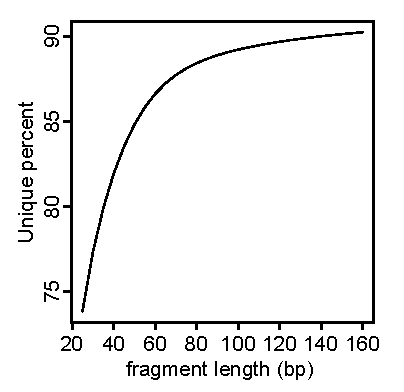
\includegraphics{ch4_fig1.pdf}
\caption{The fraction of genome that is uniquely mappable decreases with
          fragment length.}
\label{dzones}
\end{figure}

%% How will our method remove the current barrier
We propose a method to estimate the number of fragments on a SMURF-seq
read. We define a score function for aligning a SMURF-seq read, study
the distribution of aligning reads and reference generated at random,
and estimate the number of fragments in a SMURF-seq read by comparing
its alignment score with the distribution of aligning random reads for
all possible fragmentations of a read. Then we show the accuracy of our
method using from simulated genomes and SMURF-seq reads. Further, we
empirically show that this method could also be used with a general
score function.

%%%%% How will this improve scientific capacity and knowledge




%%%%%%%%%%%%%%%%%%%%%%%%%%%%%%%%%%%%%%%%%%%%%%%%%%%%%%%%%%%%%%%%%%%%%%%%
%%%%%%%%%%%%%%%%%%%%%%%%%%%%%%%%%%%%%%%%%%%%%%%%%%%%%%%%%%%%%%%%%%%%%%%%
%%%%%%%%%%%%%%%%%%%%%%%%%%%%%%%%%%%%%%%%%%%%%%%%%%%%%%%%%%%%%%%%%%%%%%%%
\section{Background}
In the early days of DNA sequencing, as the number of nucleotides
sequenced grew, comparison of DNA sequences became an indispensable tool
to a biologist.
%
DNA sequence comparison can be broadly classified into global alignment
\cite{needleman1970general} and local alignment
\cite{smith1981identification}. A global alignment seeks an optimal
alignment between two sequences such that each base of one sequence is
aligned to each base of the other sequences. On the other hand, a local
alignment seeks an optimal alignment between any subsequences of the
sequences being compared.

Comparison of two sequences, even unrelated or random sequences, always
produces an optimal alignment. This motivated the development of
approaches to differentiate a ``meaningful'' alignment from alignment of
unrelated sequences. These methods determine the significance of an
alignment by comparing the alignment score with a null distribution of
alignment scores of unrelated sequences. Determining the appropriate null
distribution was the subject of an enormous amount of research, some of
which are summarized below.

%% Simulation studies
In the context of local alignment, at the time of the initial studies on
the score distribution of unrelated sequences, mathematical tools to
understand the null distributions were still lacking, and these studies
relied on empirical distributions generated from aligning unrelated
sequences.
%%
In \cite{smith1985statistical}, it is shown that the similarity score is
proportional to the logarithm of the length of the sequences being
compared, and the standard deviation is independent of the sequence
length. The significance of an alignment was determined from the number
of standard deviations over mean of the alignment score.
%% Dependence on sequence properties
These studies \cite{lipman1984statistical} also highlight that the
statistical properties \cite{smith1983statistical}, such as nucleotide
frequencies or codon usage, of the sequences affect the distribution of
the alignment scores.  Generating a null distribution from an incorrect
model could lead to an alignment of unrelated sequences being dubiously
declared significant. Several methods are available to generate random
sequences preserving these statistical properties
\cite{fitch1983random,altschul1985significance}.

%% Mike's approach: coin tossing
Erdos and Renyi \cite{erdos1975length} presented results for the length
of the longest headrun in a the first $n$ tosses of a biased coin.  The
length of the longest headrun in coin tosses is equivalent to the number
of matches between two DNA sequences when shifts in the starting and
ending positions of the sequences are not allowed, with the probability
of head equal to the probability of match between letters of the DNA
alphabet.
% coin tossing with shifts and fixed mismatches.
In \cite{arratia1985erdos}, this is generalized to matches between DNA
sequences, while allowing shifts. These results indicate that allowing
shifts doubles the length of the longest headrun. Results for the
longest headrun allowing for up to $k$ mismatches and sequences
generated from a Markov chain are also considered.
% EVD approximation
In \cite{arratia1986extreme,gordon1986extreme} the distribution of the
longest matches is shown to a have an extreme value distribution with
mean that is proportional to the logarithm of the sequences lengths and
variance independent of sequence length. Here, when considering only
matches, the asymptotic extreme value distribution is shown by
considering a maximum of geometric distributions, and when mismatches
are allowed, it is shown by considering a maximum of negative binomial
distributions.
% poisson approximation
An alternate approach is a Poisson approximation for the distribution of
the longest match \cite{arratia1989erdos}.

%% Dembo and Karlin's approach
An crutial aspect of in aligning nucleic acid and protein sequnces is
usesing the appropriate score function. For example, PAM and Dayoff
matrices is used for protien sequcences \cite{}, and xxx is used for DNA
sequences \cite{}.  The score function used alters the score of the
aligned sequences and thus the alignment score distrubution of unaligned
sequences.
% Headrun approach does not consider score function
However, the approach based on the length of the headruns does not
consider the score function used for an alignmt.
%
In \cite{}, it is shown that the score distrubution of aligning
unrelated sequences for any score function (that has at least one
positive score and the expected score is negative) has the form of an
extreme value distribution, and and explicit formulas that its paramets
are provided.
% distribution of letters, and log-odds ratio



%% alignment allowing gaps

%% BLAST

%% Profile alignment

%% Global alignment score distribution

%% Differneces between these and the k=1 frag id problem




%% local alignment
% The local alignment score distribution has been studied extensively,
% especially in the context of BLAST score statistics
% \cite{altschul1990basic,altschul199627}.  The distribution of the local
% alignment score is well approximated by the extreme value distribution
% (EVD) \cite{karlin1990methods,
% karlin1990statistical,dembo1994limit,dembo1991strong}.

% It has also been shown that the distribution of the maximum score
% obtained when a profile sequence is aligned to all possible positions of
% a random sequence has a limiting extreme value distribution
% \cite{goldstein1994approximations}.


%%%%%%%%%%%%%%%%%%%%%%%%%%%%%%%%%%%%%%%%%%%%%%%%%%%%%%%%%%%%%%%%%%%%%%%%
%%%%%%%%%%%%%%%%%%%%%%%%%%%%%%%%%%%%%%%%%%%%%%%%%%%%%%%%%%%%%%%%%%%%%%%%
%%%%%%%%%%%%%%%%%%%%%%%%%%%%%%%%%%%%%%%%%%%%%%%%%%%%%%%%%%%%%%%%%%%%%%%%
\section{Fragment Identification problem}
%% string properties
Let $\Sigma$ be an alphabet. A string $X$ is a sequence of letters $a_0
a_1 \dots a_{n-1}$, where $a_i \in \Sigma$; $|X|$ denotes the length of
the string $X$; and $X[i \dots j] = a_i \dots a_{j-1}$ is a substring of
$X$.

%% reference string
The reference string $T$ is generated from the DNA alphabet $\Sigma =
\{A, T, G, C\}$, with $|T| = n$.
%% SMURF-seq string
A SMURF-seq read $S$ is generated by concatenating substrings (called
fragments) of $T$, with no information available \textit{a priori} about
the number, length, orientation (forward or reverse-complement), and the
position on $T$ of these fragments.  Further, $S$ contains sequencing
errors with a rate $\rho$. Let $|S| = m$ and $m \ll n$.

%% fragment set
A fragment set $P$ is an set of start locations of fragments on $S$. $P
\subset \{0 \dots m-1\}$ and $|P| = k$, with the rule that $0$ is in $P$
always.
%%
By convention we consider the set $P$ to be ordered such that if $i < j$
then $P_i < P_j$.
%%
For a fragment set $P$, $\sum_{i = 1}^{k} P_{i+1} - P_i = m$ and we say
that the $i^{\text{th}}$ of $S$ is the substring $S[P_i \dots P_{i+1}]$,
with $P_{k+1} = m$.

%% fragment identification problem
For a given $T$ and $S$, the fragment identification problem is to
determine the elements of the fragment set $P$ such that it corresponds
to the start locations of fragments contained in $S$.



%%%%%%%%%%%%%%%%%%%%%%%%%%%%%%%%%%%%%%%%%%%%%%%%%%%%%%%%%%%%%%%%%%%%%%%%
%%%%%%%%%%%%%%%%%%%%%%%%%%%%%%%%%%%%%%%%%%%%%%%%%%%%%%%%%%%%%%%%%%%%%%%%
%%%%%%%%%%%%%%%%%%%%%%%%%%%%%%%%%%%%%%%%%%%%%%%%%%%%%%%%%%%%%%%%%%%%%%%%
\section{Approach to the fragment identification problem}
%% Any k gives a score. Highest score does not correspond to the opt.
By the score function defined above, to determine the elements of the
fragment set $P$, requires the knowledge of the number of fragments $k$
and this is not known \textit{a priori}. Further, the $k$ that maximizes
the score function would almost never correspond to the optimal fragment
set. As an example, taking $k=m-1$ which corresponds to taking each base
as a fragment would maximize the score, however, this is a non-sensical
alignment.
%% So we need a way to detemine the optimal k.
Therefore, we require a approach to determine the optimal $k$.

%% Differences with the local alignment approach
% We are interested in opt frags, and not significant alignment
However, the fragment identification problem differs from the local
alignment problem in a crucial manner. For the fragment identification
problem we have the reference genome, and it is assumed that the reads
always arise from this genome; the score distribution of sequences
generated at random is used to determine the optimal number of
fragments, and not ``meaningful'' alignments.

We approach the fragment identification problem by defining a score
function as follows:
%% score function
For a given fragment set $P$, we define the score of aligning $S$ to $T$
as: \[score_T(S,P) = \sum_{i=1}^{k} \max\{score(T[u \dots v], S[P_i
\dots P_{i+1}]): 0 \leq u < v \leq n\}.\] This allows us to
consider the fragment identification problem as two inter-related
problems: (1) Determining $k$, the size of the fragment set, and (2)
given $k$, determining the elements of $P$ such that $score_T(S, P)$ is
maximized.

%% Brief description of approach


%%%%%%%%%%%%%%%%%%%%%%%%%%%%%%%%%%%%%%%%%%%%%%%%%%%%%%%%%%%%%%%%%%%%%%%%
%%%%%%%%%%%%%%%%%%%%%%%%%%%%%%%%%%%%%%%%%%%%%%%%%%%%%%%%%%%%%%%%%%%%%%%%
%%%%%%%%%%%%%%%%%%%%%%%%%%%%%%%%%%%%%%%%%%%%%%%%%%%%%%%%%%%%%%%%%%%%%%%%
\section{Score distribution under a random model}
\paragraph{Problem definition for a random model:}
The strings $T$ and $S$ are generated by drawing letters independently
from the same distribution from an alphabet $a \in \Sigma$ with
probability $p_a$ such that $\sum_{a \in \Sigma} p_a = 1$.
For a given fragment set $P$, what is the distribution of $score_T(S,
P)$?


\subsection{Score distribution of one fragment}
%% How fragment identification problem differs from these
The distribution of $score_T(S,1)$ differs from the local alignment as
we require an end-to-end alignment of $S$ to a substring of $T$. It also
differs from the profile score distribution since the letters of $S$ are
generated at random.

%% distribution for k = 1
Based on these results, the distribution of $score_T(S,1)$ is likely to
follow an extreme value distribution. The heuristic is as follows.
% heuristic of proof
Let $X_j$ denote the score of aligning $S$ with $T[j \dots j+m-1]$, then
\[X_j = \sum_{i=0}^{m-1} score(S[i],T[j+i]), j = 0, \dots, n-m+1.\]
Since the letters of T and S are iid, we have \[X_j \sim binom(m,p)\]
where $p = \sum_{a=\Sigma} p_a^2$.  For a large enough $m$, $X_j$ can
be approximated by a normal distribution as \[X_j \sim N(mp, mp(1-p)).
\] $score_T(S,1)$ is the maximum score over all positions in $T$,
\[score_T(S,1) = \max_{0 \leq j \leq n-m+1} X_j.\] $score_T(S,1)$ is a
maximum of normal distributions, which follows an extreme value
distribution \cite{kotz2000extreme}.
%% m-dependence
Here, we have a dependence between $X_j$ and $X_k$ for $|j - k| < m$.

%% distribution and qq plot

%% Distribution as a function of fragment length

%% Distribution as a function of genome length

\subsection{Score distribution for a given fragment set}


\subsection{Score distribution for an unknown fragment set}


%%%%%%%%%%%%%%%%%%%%%%%%%%%%%%%%%%%%%%%%%%%%%%%%%%%%%%%%%%%%%%%%%%%%%%%%
%%%%%%%%%%%%%%%%%%%%%%%%%%%%%%%%%%%%%%%%%%%%%%%%%%%%%%%%%%%%%%%%%%%%%%%%
%%%%%%%%%%%%%%%%%%%%%%%%%%%%%%%%%%%%%%%%%%%%%%%%%%%%%%%%%%%%%%%%%%%%%%%%
\section{Identifying optimal fragment boundaries}



%%%%%%%%%%%%%%%%%%%%%%%%%%%%%%%%%%%%%%%%%%%%%%%%%%%%%%%%%%%%%%%%%%%%%%%%
%%%%%%%%%%%%%%%%%%%%%%%%%%%%%%%%%%%%%%%%%%%%%%%%%%%%%%%%%%%%%%%%%%%%%%%%
%%%%%%%%%%%%%%%%%%%%%%%%%%%%%%%%%%%%%%%%%%%%%%%%%%%%%%%%%%%%%%%%%%%%%%%%
\section{Estimating the number of fragments}




%%%%%%%%%%%%%%%%%%%%%%%%%%%%%%%%%%%%%%%%%%%%%%%%%%%%%%%%%%%%%%%%%%%%%%%%
%%%%%%%%%%%%%%%%%%%%%%%%%%%%%%%%%%%%%%%%%%%%%%%%%%%%%%%%%%%%%%%%%%%%%%%%
%%%%%%%%%%%%%%%%%%%%%%%%%%%%%%%%%%%%%%%%%%%%%%%%%%%%%%%%%%%%%%%%%%%%%%%%
\section{Results}


\subsection{Exact matching reads}

\subsection{Reads with mismatches}
